\documentclass[12pt, letterpaper, twoside]{article}
\usepackage[utf8]{inputenc}
\usepackage{amsfonts}
\usepackage{amsmath}
\usepackage{amssymb}
\usepackage{ifthen}
\usepackage{fancyhdr}
\usepackage{tikz}
\usepackage{csc}
\usepackage{listings}
\usepackage{xcolor}
\usepackage{pgfplots}

\definecolor{codegreen}{rgb}{0,0.6,0}
\definecolor{codegray}{rgb}{0.5,0.5,0.5}
\definecolor{codepurple}{rgb}{0.58,0,0.82}
\definecolor{backcolour}{rgb}{0.95,0.95,0.92}

\lstdefinestyle{mystyle}{
    backgroundcolor=\color{backcolour},   
    commentstyle=\color{codegreen},
    keywordstyle=\color{magenta},
    numberstyle=\tiny\color{codegray},
    stringstyle=\color{codepurple},
    basicstyle=\ttfamily\footnotesize,
    breakatwhitespace=false,         
    breaklines=true,                 
    captionpos=b,                    
    keepspaces=true,                 
    numbers=left,                    
    numbersep=5pt,                  
    showspaces=false,                
    showstringspaces=false,
    showtabs=false,                  
    tabsize=2
}

\lstset{style=mystyle}

\oddsidemargin=.2in
\evensidemargin=.2in
\textwidth=6in
\topmargin=0in
\textheight=9.0in
\parskip=.07in
\parindent=0in
\pagestyle{fancy}



\begin{document}

\setheader{CSC165}{Lecture 13}{Arthur Gao}{}{}{}

\section{An Example}
Examine the code:
\begin{lstlisting}[language=Python]
def twisty(n: int) -> None:     #Precondition: n >= 1
    while n > 1:
        if n % 2 == 0:
            n = n//2
        else:
            n = 2 * n - 2
\end{lstlisting}

Examining the function above with the following inputs to \code{n}:

\begin{center}
    \begin{tabular}{c c}
        \hline
        \code{n} &Values of \code{n}\\
        \hline
        1 &1\\
        2 &2, 1\\
        3 &3, 4, 2, 1\\
        4 &4, 2, 1\\
        5 &5, 8, 4, 2, 1\\
        165 &165, 328
    \end{tabular}
\end{center}
We see:
\begin{itemize}
    \item if \code{n} is odd, then $2 * n - 2$ is even, and therefore after 2 iterations, it's $n - 1$
    \item If \code{n} is even, \emph{and $n > 1$} then after 1 iteration it's $\frac{n}{2} \le n - 1$
\end{itemize}

Therefore, we note that every 1 or 2 iterations, n goes down by at least $1$ and concequently the program
must terminate after at most $2n$ iterations. In this way $RT_{twisty} \in \bigO(n)$

\subsection{Non integer inputs}
\begin{lstlisting}[language=Python]
def is_pal(s: str) -> bool:
    for i in range(len(s)):
        if s[i] != s[len(s) - 1 - i]:
            return False
    return True
\end{lstlisting}
We note that the runtime is a function of the input - which is a string - so we must determine a method
for measuring the input in natural numbers. In this case, we use the size/length.

Potential worst case runtime of \code{is\_pal} given different sized inputs\\
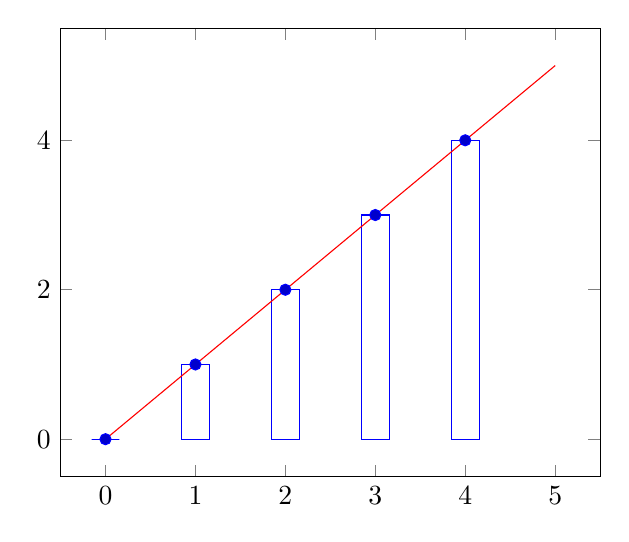
\begin{tikzpicture}
    \begin{axis}
        \addplot+[ybar] coordinates {
            (0,0) 
            (1,1)
            (2,2) 
            (3,3) 
            (4,4)
        };
        \addplot[domain=0:5, color=red]{x};
    \end{axis}
\end{tikzpicture}

For $n \in \N,$ let $\mathcal{I}_n = \{s \in str : |s| = n\}$
Let $WC(n) = max \{RT(s): s \in \mathcal{I}_n\}$

Let $E \subseteq \R $ and $E$ has a maximum and $l \le max E \le u$

\hspace*{10mm}it's worth noting that $maxE \in E$ and $\forall e \in E, e \le maxE$
\end {document}